\documentclass{article}
\usepackage{fullpage} % Package to use full page
\usepackage{parskip} % Package to tweak paragraph skipping
\usepackage{tikz} % Package for drawing
\usepackage{amsmath}
\usepackage{hyperref}
\usepackage{enumitem}
\usepackage{float}
\usepackage{ upgreek }
\usepackage[explicit]{titlesec}
\usepackage{graphicx}
\usepackage {verbatim}
\newcommand{\RNum}[1]{\uppercase\expandafter{\romannumeral #1\relax}}
%\titleformat{\section}{\normalfont\Large\bfseries}{}{0em}{#1\ \thesection}

\title{Inlämning 4 \\ Objektorienterad programmering med Java}
\author{Emil Björklund - embj3739 \\ emilbjorklund@live.com}


\begin{document}

\maketitle 
\newpage

\section{Inledning}
\begin {itemize}
\item IDE: Visual Studio Code
\item Java verision: JDK 8 update 191
\item OS: MacOS Mojave
\end{itemize}

\textbf{Note.} Källkoden bifogas i separat .zip som finns i inlämningen.

\section{Kom-igång}
Programmet staras genom att öppna Pasture.bin från terminalen eller liknande.
Innan simuleringen startar kan användaren välja att fylla i dom tomma fälten till höger för att ändra vald parameter.
För att bekräfta ändringar av parametrar trycker användaren på knappen Custom och sedan Start för att starta simuleringen.
Om användaren vill använda sig av standrard parametrar tycker användaren på knappen Default följt av Start.
När simuleringen är avslutad och användaren trycka på knappen Exit kan an välja att spara resultatet till textfil för att föra statistik.
\\
Tips! Kolla javadoc för mer information.
\section{Struktur}
\begin{figure}[H]
  \centering
    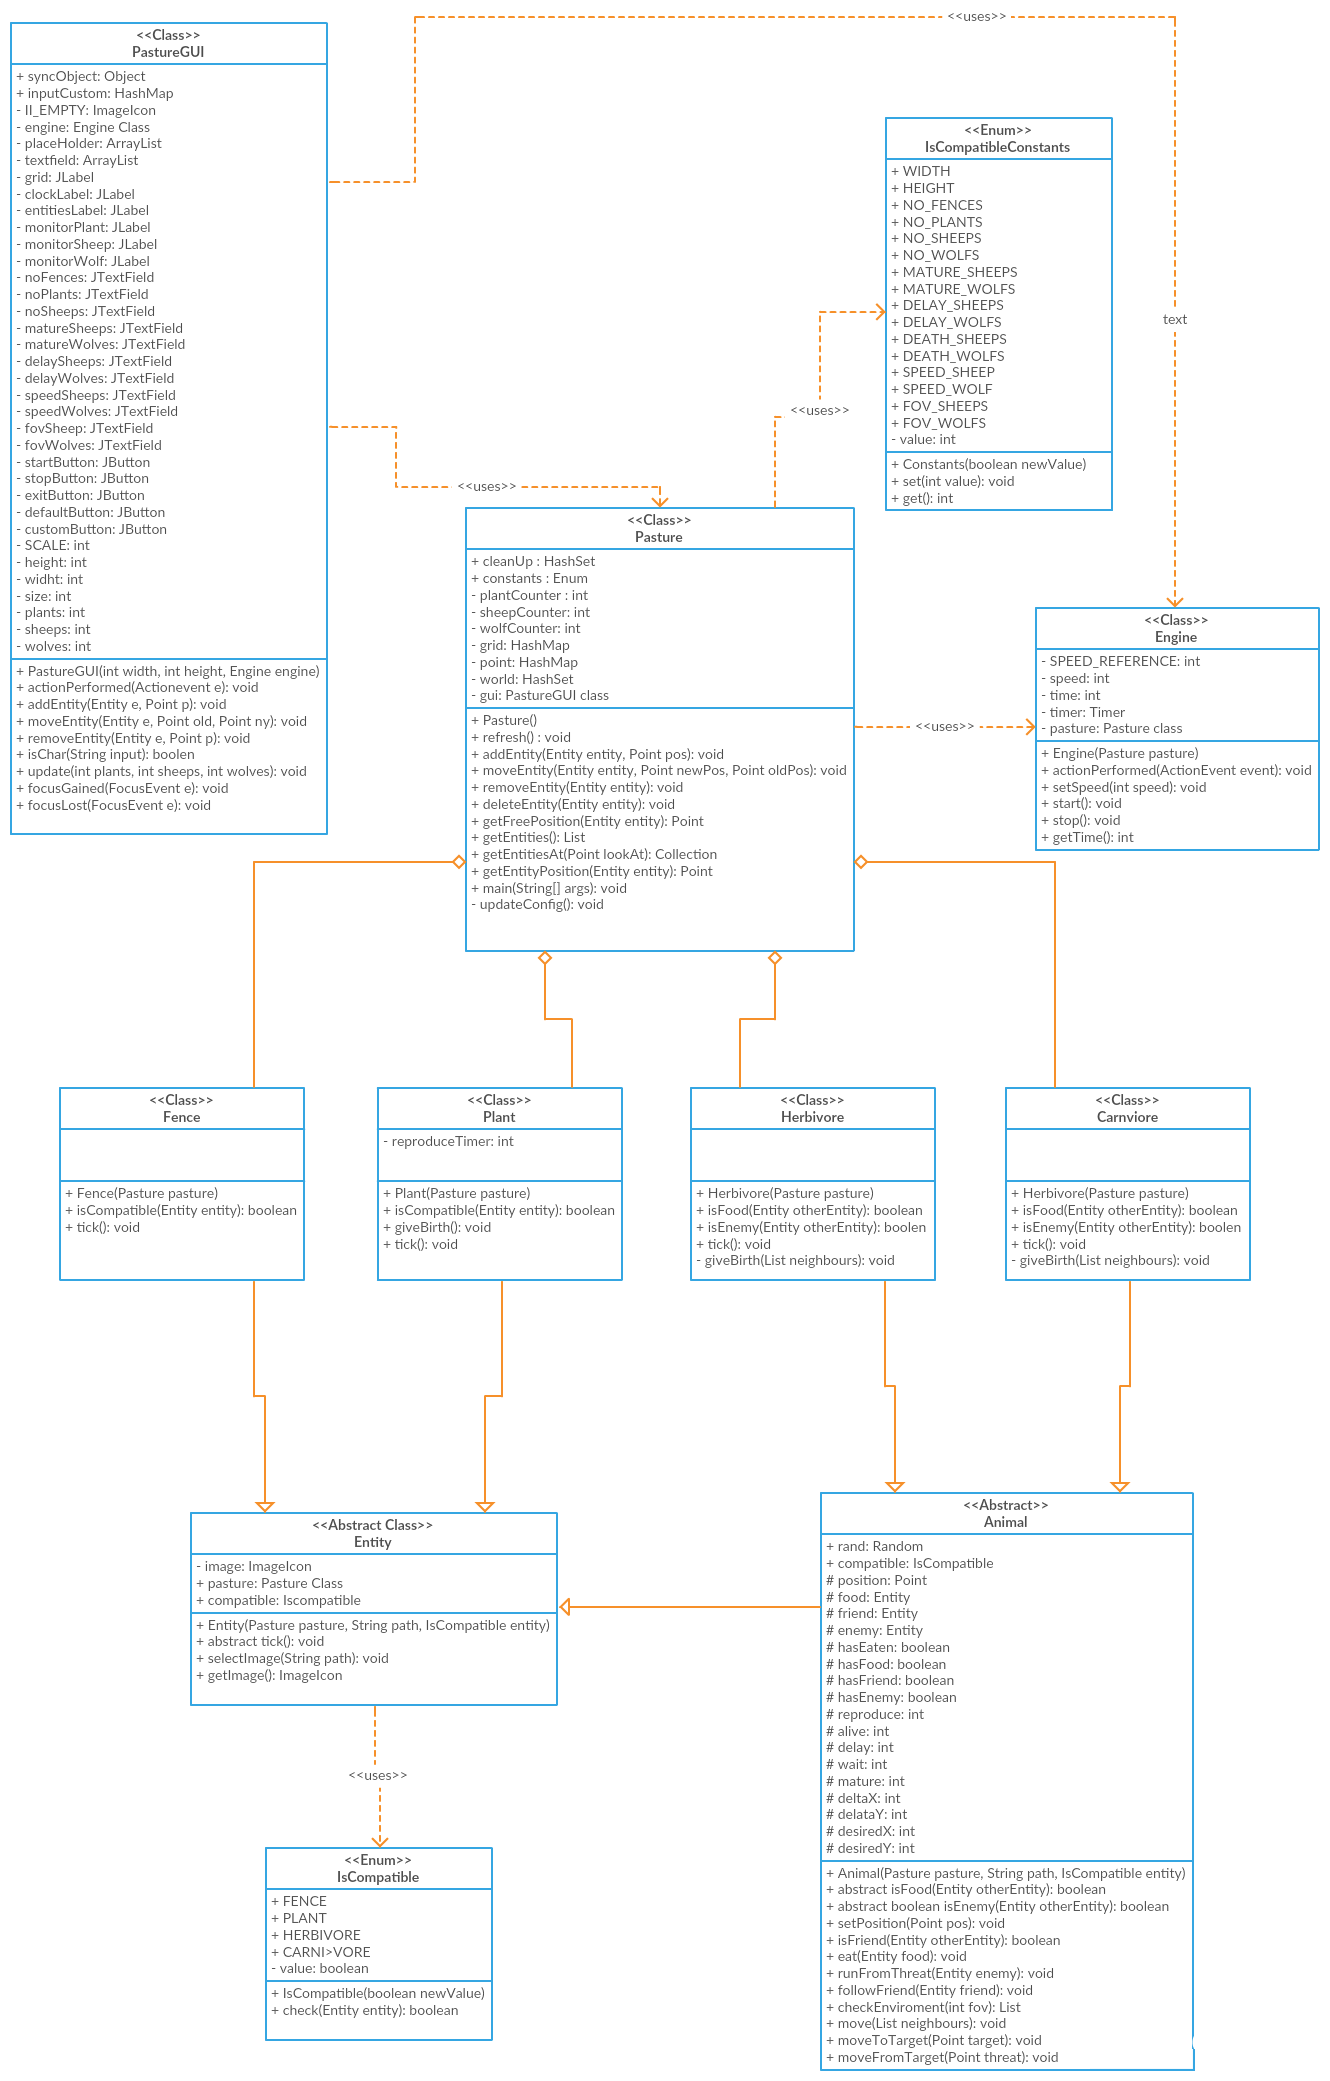
\includegraphics[width=0.8\linewidth]{uml.png}
  \label{fig:1}
\end{figure}

\subsection{Class Pasture}
Klassen Pasture har main konstruktorn och har som främsta uppgift att lagra, ta bort och flytta runt objekt i fönstret.
Klassen har bland annat ett "Set" med namnet world. Fördelen med typen Set är att Set inte tillåter några dublicerade element
vilket möjliggör att alla objekt i "hagen" kan lagras på ett säkert sätt. Det finns även två HashSet för att koppla x och y kordinater med vilka objekt som befinner sig på punkten.
Samt  koppla varje ensklit objekt med en given position. Fördelen med ett HashSet är att varje element kopplas till en nyckel, t.ex.
om nyckeln är position så kommer HasMap.get() retunera alla objekt på denna position.
Genom att ta bort ett objekt från en punkt och sedan lägga till samma objekt på en ny punkt kan objekten i simuleringen röra på sig.
Slutligen har även klassen Pasture till uppgift att deklarera objekt av andra klasser som invånarna i hagen men även PastureGUI som ritar upp fönstret och Engine som driver tiden frammåt.

\subsection{Class PastureGUI}
PastureGUI innehåller all funktionalitet som rör det grafiska. Klassen behandlar användardata och målar upp alla objekt i fönstret.
Klassen uppdaterar alla ändringar via en metod som klassen Pasture anropar.

\subsection{Class Engine}
Simuleringens motor som använder sig av en timer för att genom event som triggas på tid anropa alla tillängliga objekt i hagen från Pasture.
Alla aktiva objekt i hagen har en metod tick() som anropas från Engine.

\subsection{Class Entity}
Entity är en abstrakt klass som ligger till grund för allas objekt i hagen.
Tanken med denna klass är att metoder som manipulerar objeken i hagen skall kunna förvänta sig ett objekt som har ärvt från Entity.
Den övergripande basfunktionaliteten är implementerad här som bilden på objektet. Klassen är abstrakt eftersom metoden tick() implementeras olika beroende på vilken klass som ärver denna. 

\subsubsection{Class Animal}
Animal är precis som Entity en abtsrakt klass som alla typer av djur klasser ärver från. Denna klass i sin tur ärver från Entity. Motivationen till denna klass är att
all djur har gemensamma beteenden oavsätt art som att djuret rör sig, kollar sin omgivning, äter, följer vänner osv. Klassen är abstrakt för att vissa metoder skiljer sig åt beroende på art.
Ett får och en varg har olika matvanor och fiender som exempel.
Klassrna som repesenterar olika arter har en egen implementation av metoden tick() dock anropar alla metoden checkEnviroment() som läser av omgivningen och lagrar punkter där det finns ledigt utrymme
samt lagrar entiteter för mat, vänner och fiender.
Metoderna moveFromTarget() och moveToTarget() är väldigt lika med undantaget att resultaten blir motsatta varandra.
Logiken är som följande:
\begin{verbatim}
  public void moveToTarget(Point target) {
        deltaX = (int)target.getX() - (int)possition.getX();
        deltaY = (int)target.getY() - (int)possition.getY();

        if (deltaX != 0){
            if(deltaX > 0) desiredX = 1;
            else desiredX = -1;
        }

        if (deltaY == 0) deltaY = 0;{
            if(deltaY > 0) desiredY = 1;
            else desiredY = -1;
        }

        Point goTo = new Point((int)possition.getX()+desiredX,(int)possition.getY()+desiredY);
\end{verbatim}
Med antagandet att ett objekt endast kan röra sig en punkt per iteration så kan ej objektet direkt nå målet även om metoden checkEnviroment har hittat det.
Beroende på om skillnaden mellan objektets position och målets position är positiv eller negativ blir den nya positionen den nuvarande plus/minus 1. \\ \\
Följande bild illustrerar det generella flödet för metoden tick() som implementeras av klasserna som representerar arter.
\begin{figure}[H]
  \centering
    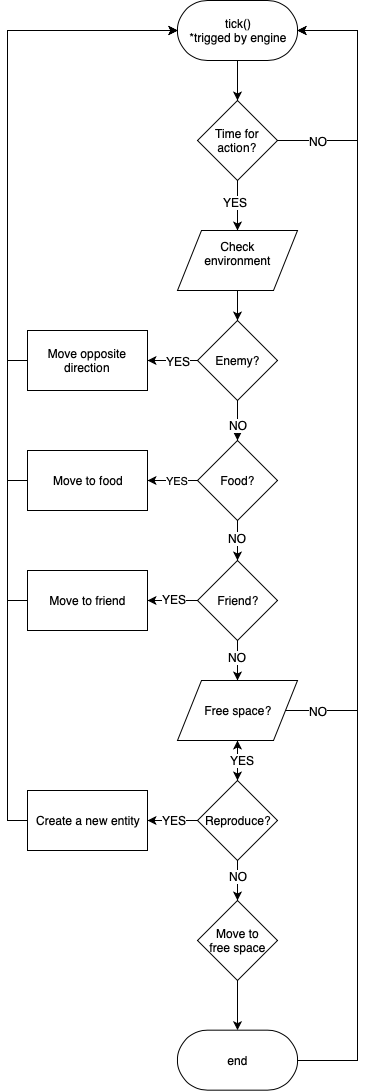
\includegraphics[width=0.2\linewidth]{tick.png}
  \label{fig:1}
\end{figure}

\paragraph{Class Carnivore}
Denna klass ärver från Animal och representerar i denna implementation Vargar men tanken är att den skall även kunna representera andra köttätare med liknande beteende.
Här implementeras dom abstrakta metoderna definierade i Animal som isFood() och isFriend().

\paragraph{Class Herbivore}
Herbivore är mycket lik klassen Carnivore men är tänkt att representera växtätande djur som i detta fall är får. Även denna klass
implementerar de abstrakta klasserna isFood() och isFriend()

\subsubsection{Class Plant}
Denna klass ärver från Entity och beskriver funktionaliteten hos ett fast objekt som gräs. Andra fasta objekt som har möjlighet till fortplantning skulle också kunna implementeras här.

\subsubsection{Class Fence}
Denna klass ärver precis som Plant från Entity och beskriver objekt som ej fortplantar sig och är fasta. Om klassen byter namn till något mer generellt så skulle objekt som stenar också lämpa sig att implementeras här.

\subsection{Enum IsCompatible}
För att alla entiteter och klasser skall veta vem som är kompatibel med vem implementerades funktionaliteten som en Enum för att enkelt kunna testa kompatibiliteten.

\subsection{Enum Constants}
För att simuleringen skall kunna ändra beteende krävs det justerbara parametrar som i vilken takt att djur får föröka sig osv. Många olika instanser behöver ha tillgång till dessa parametrar
vilket gör det användarvänligt och mer läsbart med att skapa en Enum som tillhandahåller alla konstanter. När användaren väljer att manipulera dessa konstanter så uppdateras värdera i Enum.

\section{Diskussion}
För att skapa en sådan objektorienterad lösning som möjligt ändrades strukturen många gånger i utvecklingsfasen.
Det pendlade mycket mellan att implementera vissa metoder som ett interface eller som i den nuvarande lösningen via en abstrakt klass.
Fördelen med ett interface är att den utgör ett kontrakt mellan dom olika klasserna. Eftersom bara metodhuvudet är definierat i ett interface måste
alla klasser som implementerar den utforma metoden med dess exakta funktionshuvud. Detta gör att andra klasser enkelt kan anropa metoderna och kan förvänta sig rätt argument och retur.
Fördelen med en abstrakt klass i detta fall är att klasserna som ärver den abstrakta klassen är väldigt lika och då kan icke-abstrakt funktionalitet implementeras i superklassen och dom får metoderna som är individuella kan sedan implementeras i respektive klass.
Implementationer av Enum baseras det på best practice för hanteringen av konstanter i Java.
\\
Om mer tid fanns skulle det definitivt läggas mer tid på att hitta snyggare lösningar och mer funktionalitet. 


\end{document}